\documentclass[aspectratio=169]{beamer}

\usetheme{Madrid}
\usecolortheme{seahorse}
\setbeamertemplate{navigation symbols}{}
\graphicspath{{Images/}{pre/Images/}}

\title[Learning and AI at Work]{What AI Changes in Work and Learning}
\author[Jianye Shi]{Jianye Shi}
\institute[Paris-Saclay / UVSQ]{M1 CHPS -- Universite Paris-Saclay -- UVSQ 2025/2026}
\date{March 19, 2026}

\begin{document}

\begin{frame}
  \titlepage
\end{frame}

\begin{frame}{Outline}
  \tableofcontents
\end{frame}

\section{Introduction}

\begin{frame}{AI Is Already Changing Work}
  \begin{columns}[c,totalwidth=\textwidth]
    \column{0.36\textwidth}
    {\large AI is no longer a distant possibility. It is already entering real work.}

    \vspace{1.2em}
    \begin{block}{Central Question}
      \large If AI can increasingly do difficult tasks, what exactly changes in learning?
    \end{block}

    \vspace{0.4em}
    {\scriptsize Background source: Anthropic report, March 5, 2026}
    \column{0.60\textwidth}
    \centering
    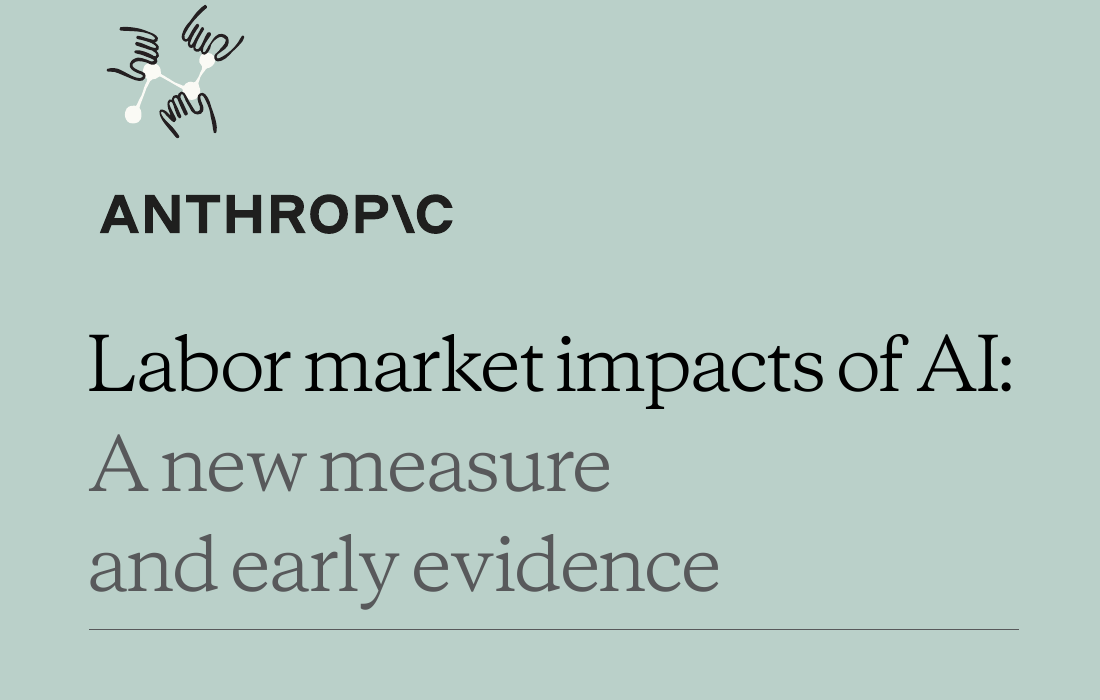
\includegraphics[width=\linewidth,height=0.72\textheight,keepaspectratio]{anthropic_cover_title.png}
  \end{columns}
\end{frame}

\section{Clarifying the Problem}

\begin{frame}[t]{Not All Change Is Replacement}
  \small
  \renewcommand{\arraystretch}{1.5}
  \centering
  \begin{tabular}{|c|l|p{0.6\textwidth}|}
    \hline
    \textbf{Level} & \textbf{Concept} & \textbf{Meaning} \\
    \hline
    Task & Exposure & AI affects the task. \\
    \hline
    Task & Automation & AI does more of the task. \\
    \hline
    Job & Transformation & The job stays, but changes. \\
    \hline
    Job & Replacement & The job is no longer needed in the same way. \\
    \hline
  \end{tabular}

  \vfill
  \begin{block}{Takeaway}
    \normalsize
    Being affected by AI is not the same as being automated by AI.\\
    And task-level change is not the same as job-level change.
  \end{block}
\end{frame}

\begin{frame}{Capability vs. Exposure}
  \begin{columns}[c,totalwidth=\textwidth]
    \column{0.35\textwidth}
    \scriptsize
    \textbf{Capability}: what AI could do in theory.

    \vspace{0.5em}
    \textbf{Exposure}: what AI is already doing in real work.

    \vspace{0.7em}
    \alert{Capability is larger than exposure.}

    \vspace{0.7em}
    Trust, regulation, habits, review costs, and responsibility slow real adoption.

    \vfill
    {\tiny Source: Anthropic, Figure 2}
    \column{0.6\textwidth}
    \centering
    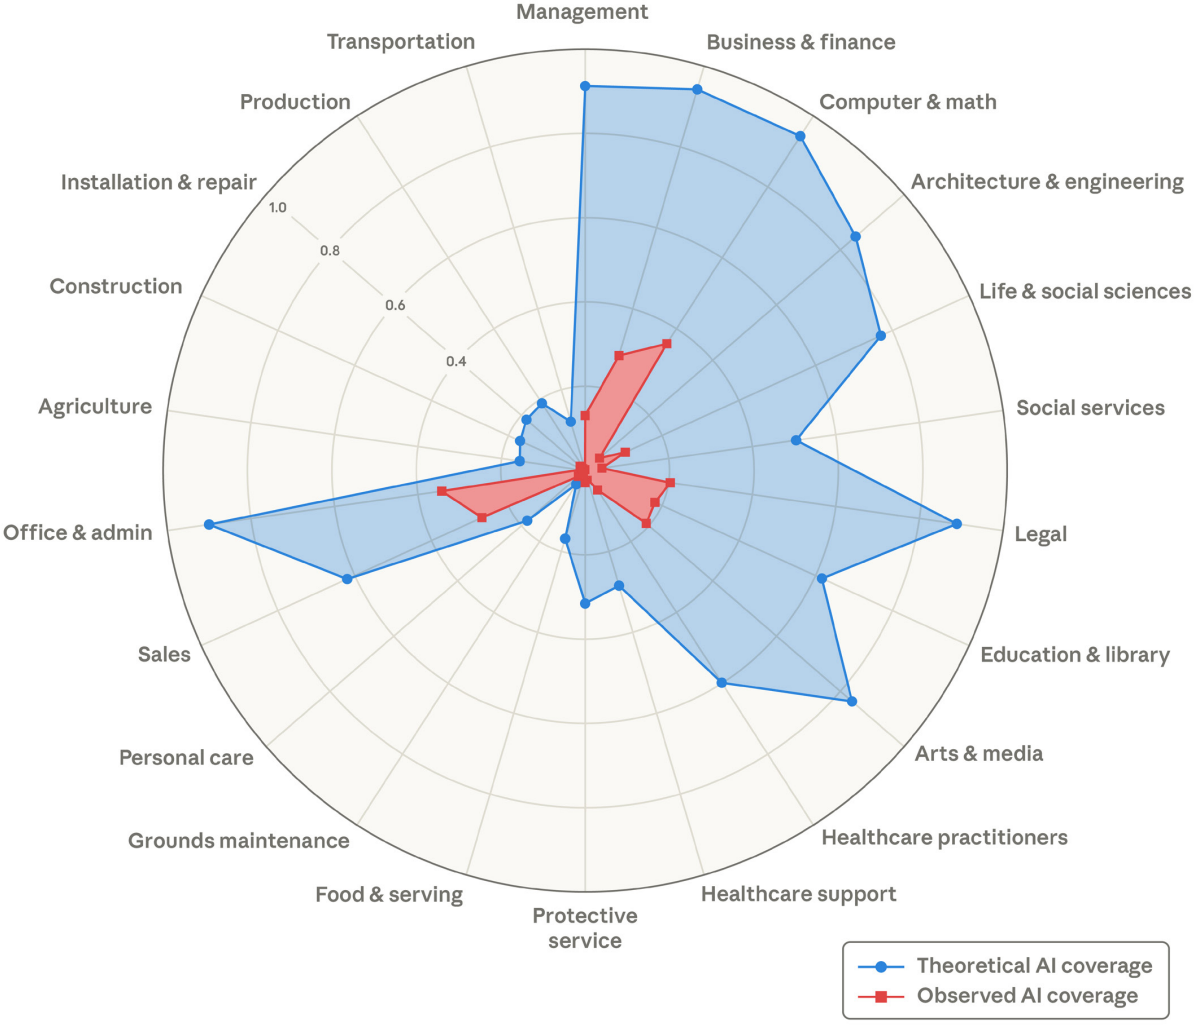
\includegraphics[width=\linewidth,height=0.89\textheight,keepaspectratio]{anthropic_fig2_trim.png}
  \end{columns}
\end{frame}

\begin{frame}{Why Some Tasks Are Affected Earlier}
  \begin{columns}[c,totalwidth=\textwidth]
    \column{0.6\textwidth}
    \small
    \begin{itemize}
      \item AI moves earlier into tasks that are easy to describe and easy to check.
      \item Adoption also comes faster when mistakes are lower-risk.
      \item Work involving human interaction, physical action, or ambiguous judgment changes more slowly.
    \end{itemize}

    \vspace{0.6em}
    \begin{block}{Main Idea}
      \small
      Exposure is uneven because tasks are uneven.
    \end{block}

    \column{0.40\textwidth}
    \centering
    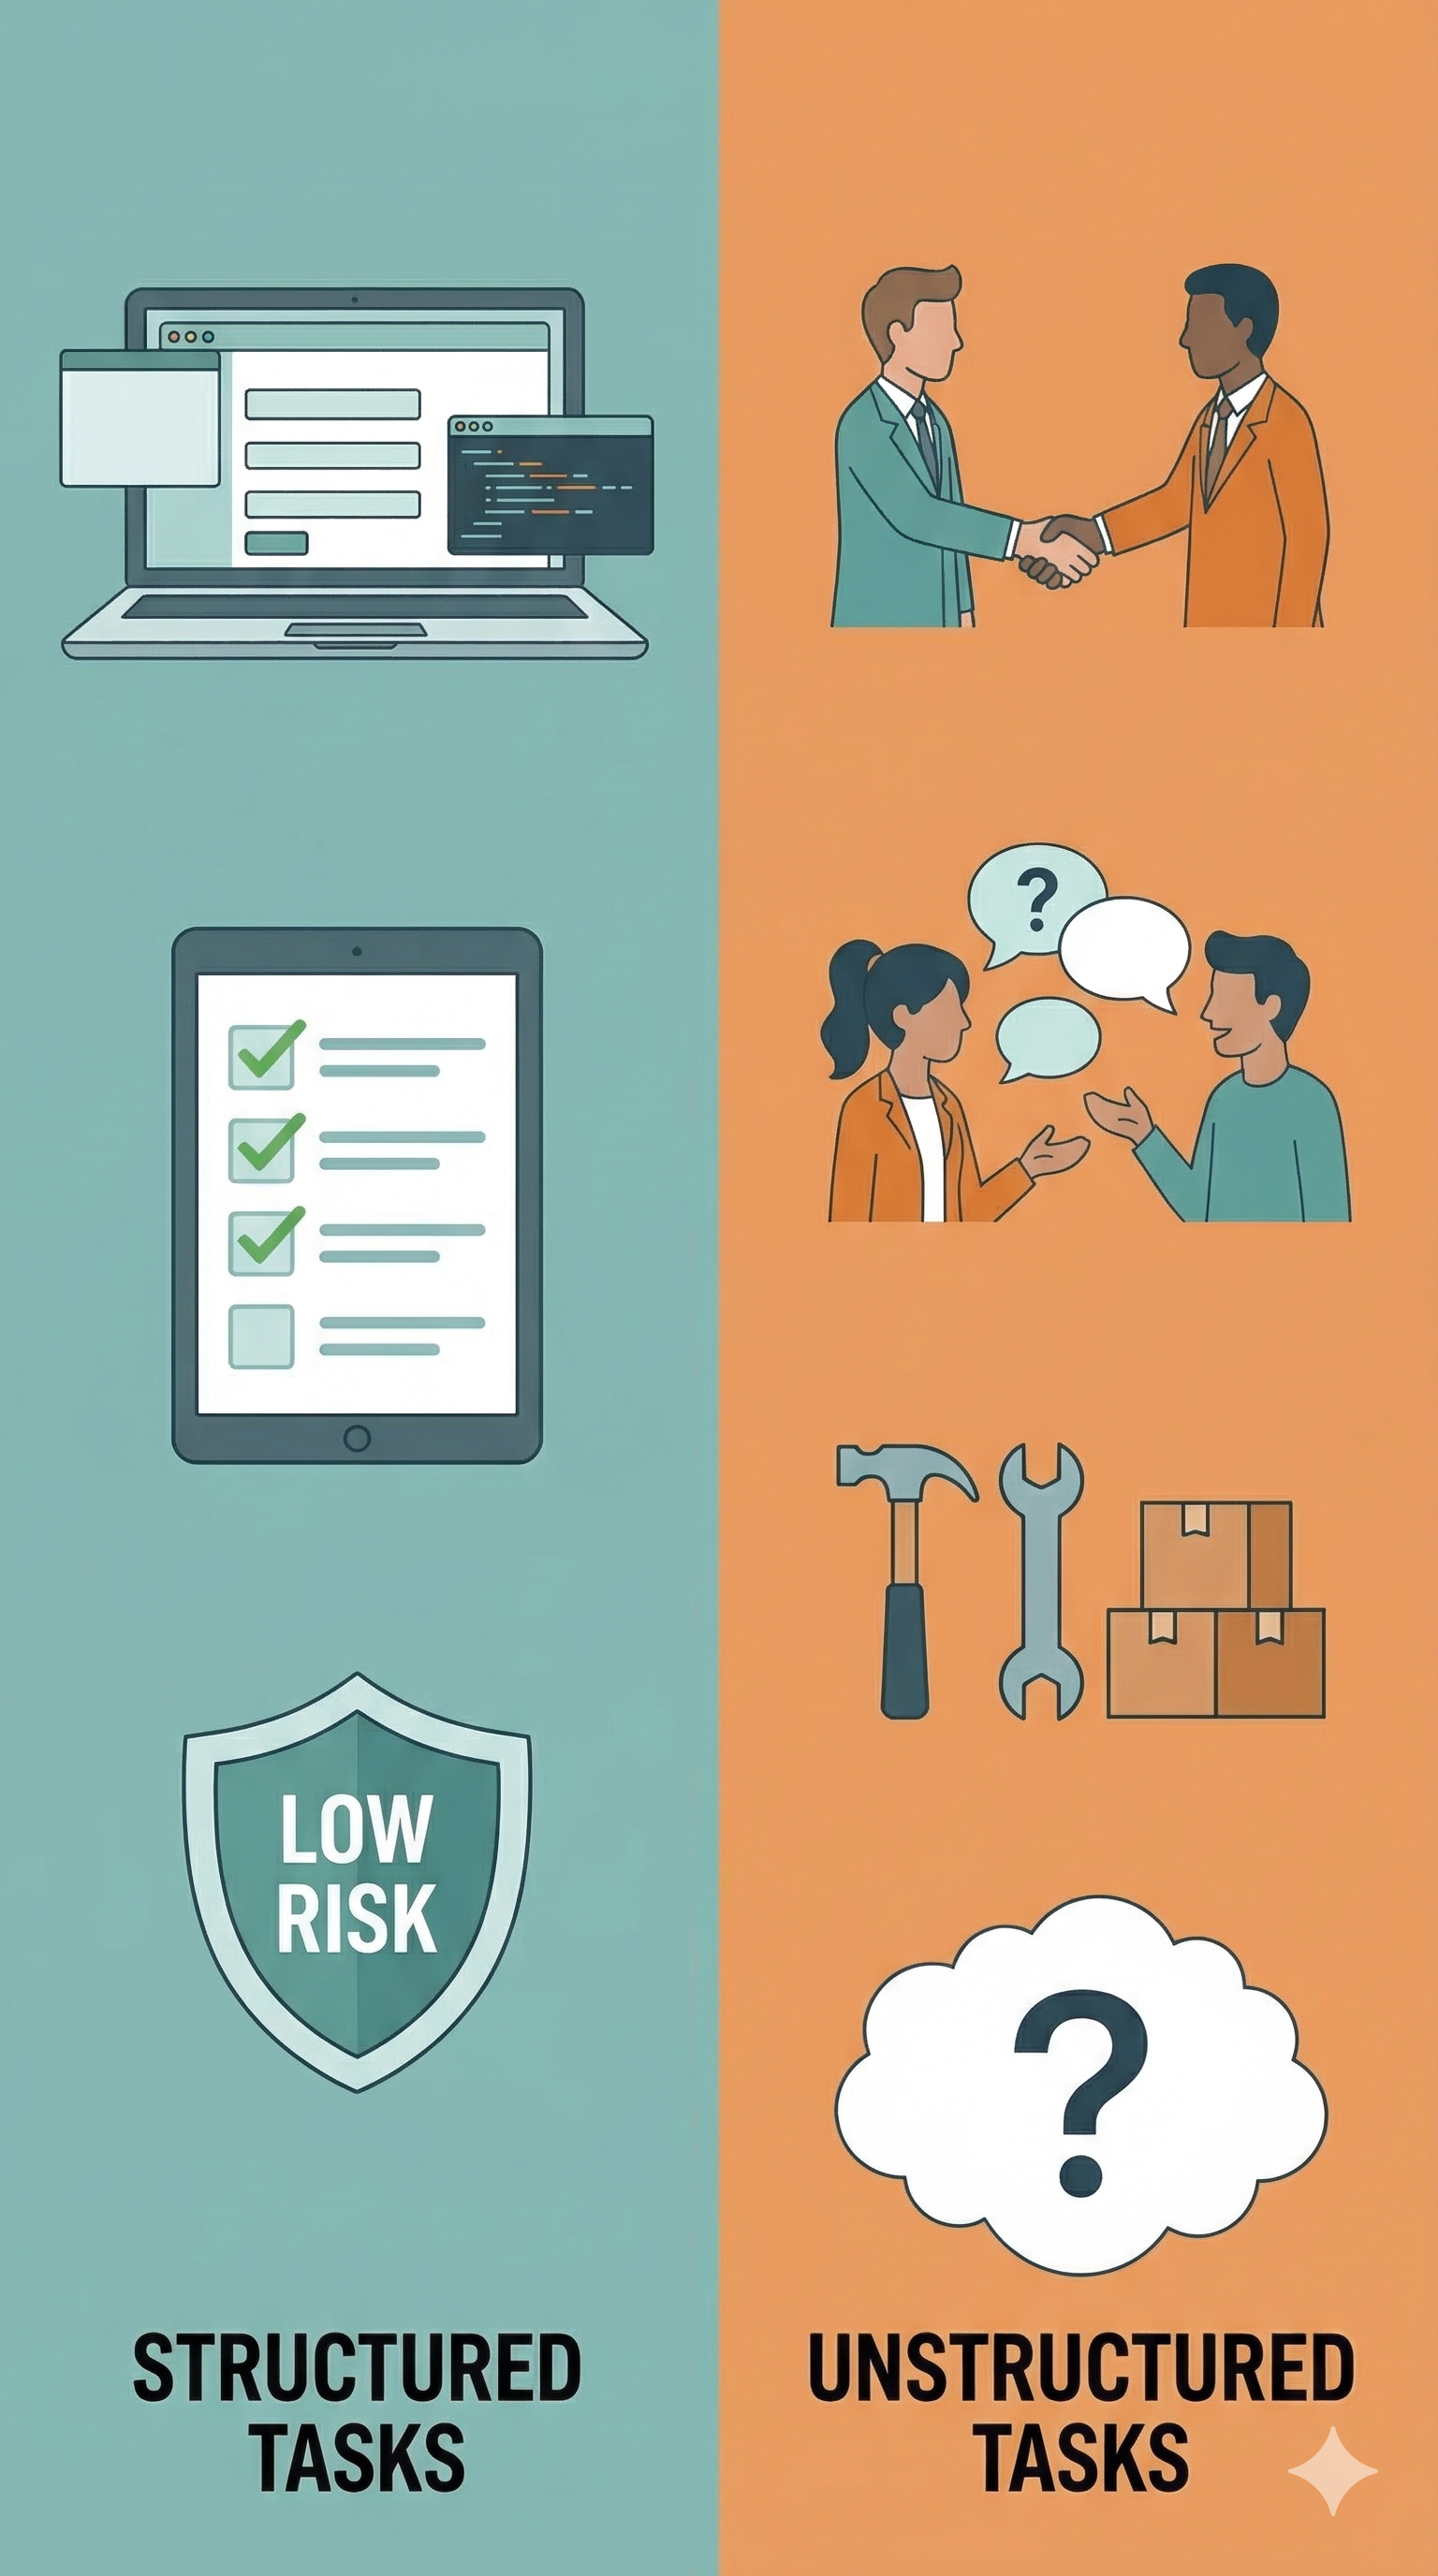
\includegraphics[width=\linewidth,height=0.78\textheight,keepaspectratio]{Gemini_Generated_Image_StructureTaskVSUnSTask.png}
  \end{columns}
\end{frame}

\section{What AI Changes in Learning}

\begin{frame}{1. Retrieval Gets Cheaper; Interpretation Does Not}
  \begin{columns}[c,totalwidth=\textwidth]
    \column{0.60\textwidth}
    \small
    \begin{itemize}
      \item AI makes answers much easier to produce.
      \item But fluent output is not the same as real understanding.
      \item Without a mental model, users may miss assumptions or errors.
    \end{itemize}

    \vspace{0.6em}
    \begin{block}{Main Shift}
      \small
      Effort moves from retrieval toward interpretation.
    \end{block}

    \column{0.40\textwidth}
    \centering
    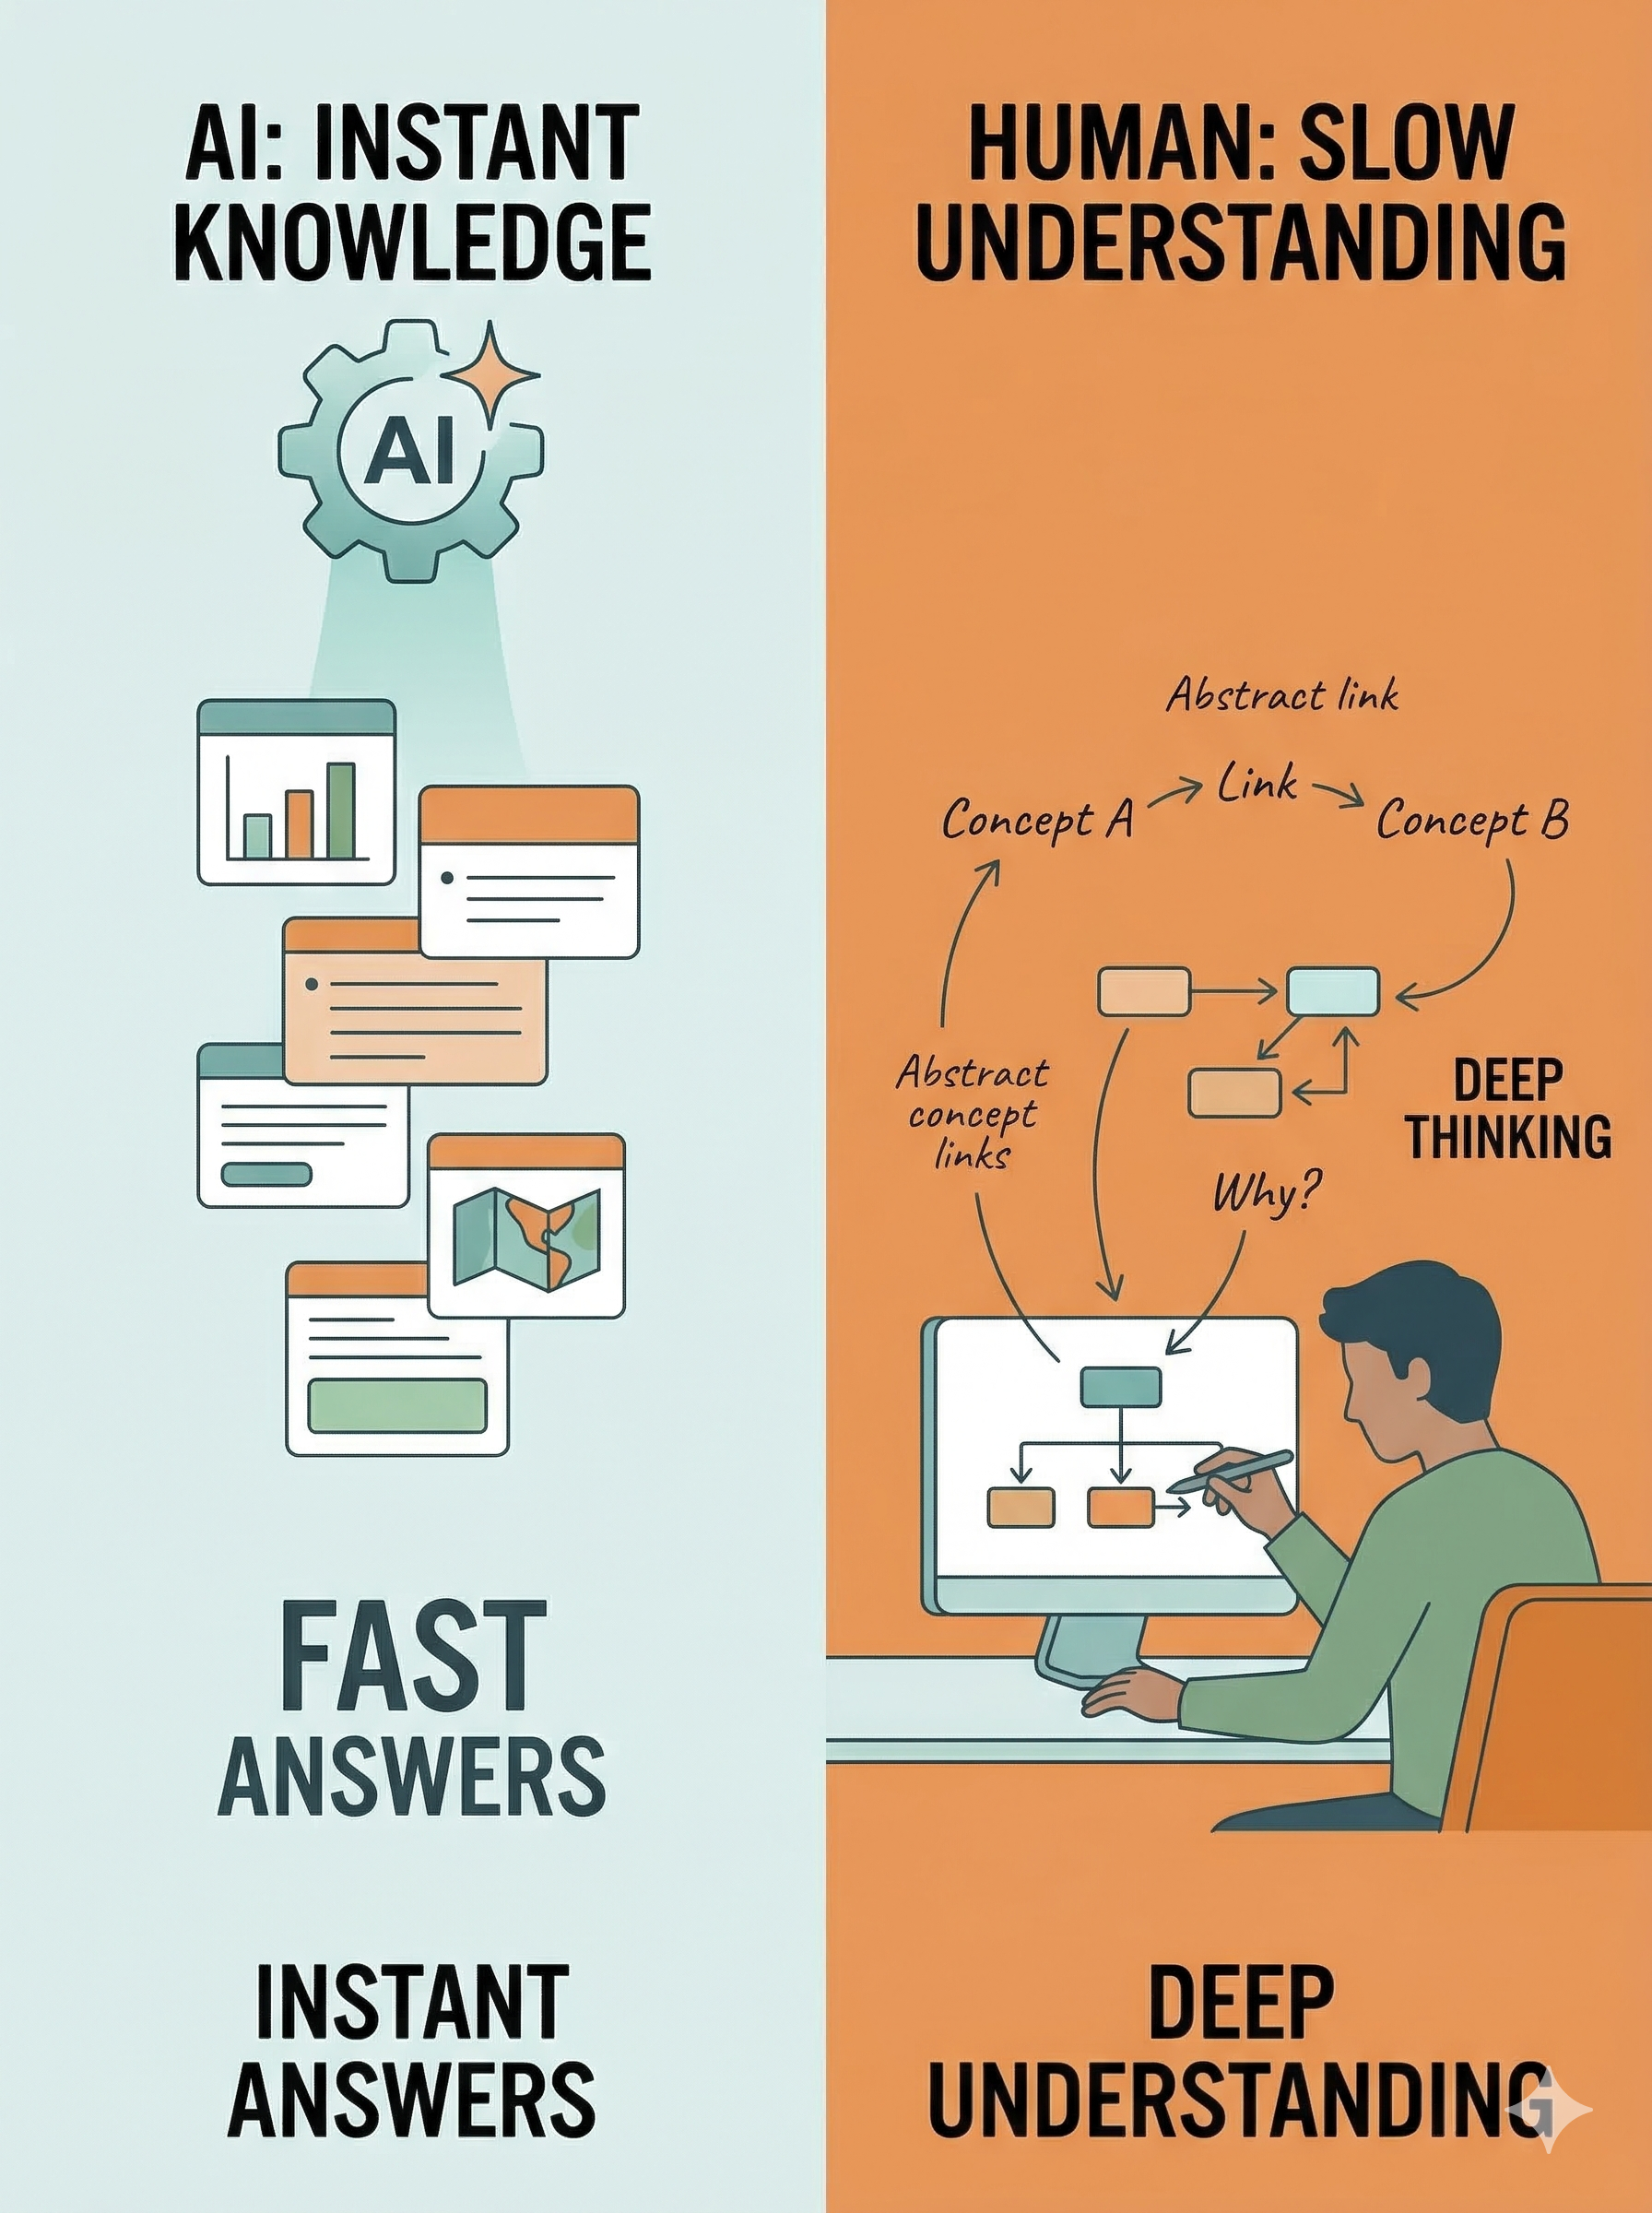
\includegraphics[width=\linewidth,height=0.78\textheight,keepaspectratio]{Gemini_Generated_Image_AnsVSUnderstand.png}
  \end{columns}
\end{frame}

\begin{frame}[c]{2. Generation Gets Cheaper; Verification Becomes the Bottleneck}
  \begin{columns}[T,totalwidth=\textwidth]
    \column{0.36\textwidth}
    \begin{block}{AI Helps}
      \centering
      \Large AI helps generate faster
    \end{block}

    \column{0.24\textwidth}
    \centering
    \vspace{1.2em}
    {\Huge $\Rightarrow$}

    \vspace{0.5em}
    {\large \alert{bottleneck shifts}}

    \column{0.36\textwidth}
    \begin{alertblock}{Human Effort Shifts To}
      \centering
      \large checking\\[0.35em]
      debugging\\[0.35em]
      judging
    \end{alertblock}
  \end{columns}

  \vfill
  \begin{block}{In Short}
    \large Generation $\rightarrow$ cheaper\\[0.35em]
    Verification $\rightarrow$ more central
  \end{block}
\end{frame}

\begin{frame}{3. What Stays Useful When Tools Keep Changing}
  \begin{columns}[c,totalwidth=\textwidth]
    \column{0.6\textwidth}
    \small
    \begin{itemize}
      \item Tool-specific familiarity loses value faster when interfaces keep changing.
      \item More abstract knowledge transfers better across tools and contexts.
      \item What lasts longer is usually foundations, not one interface.
    \end{itemize}

    \vspace{0.6em}
    \begin{block}{Main Idea}
      \small
      AI changes which knowledge stays useful over time.
    \end{block}

    \column{0.40\textwidth}
    \centering
    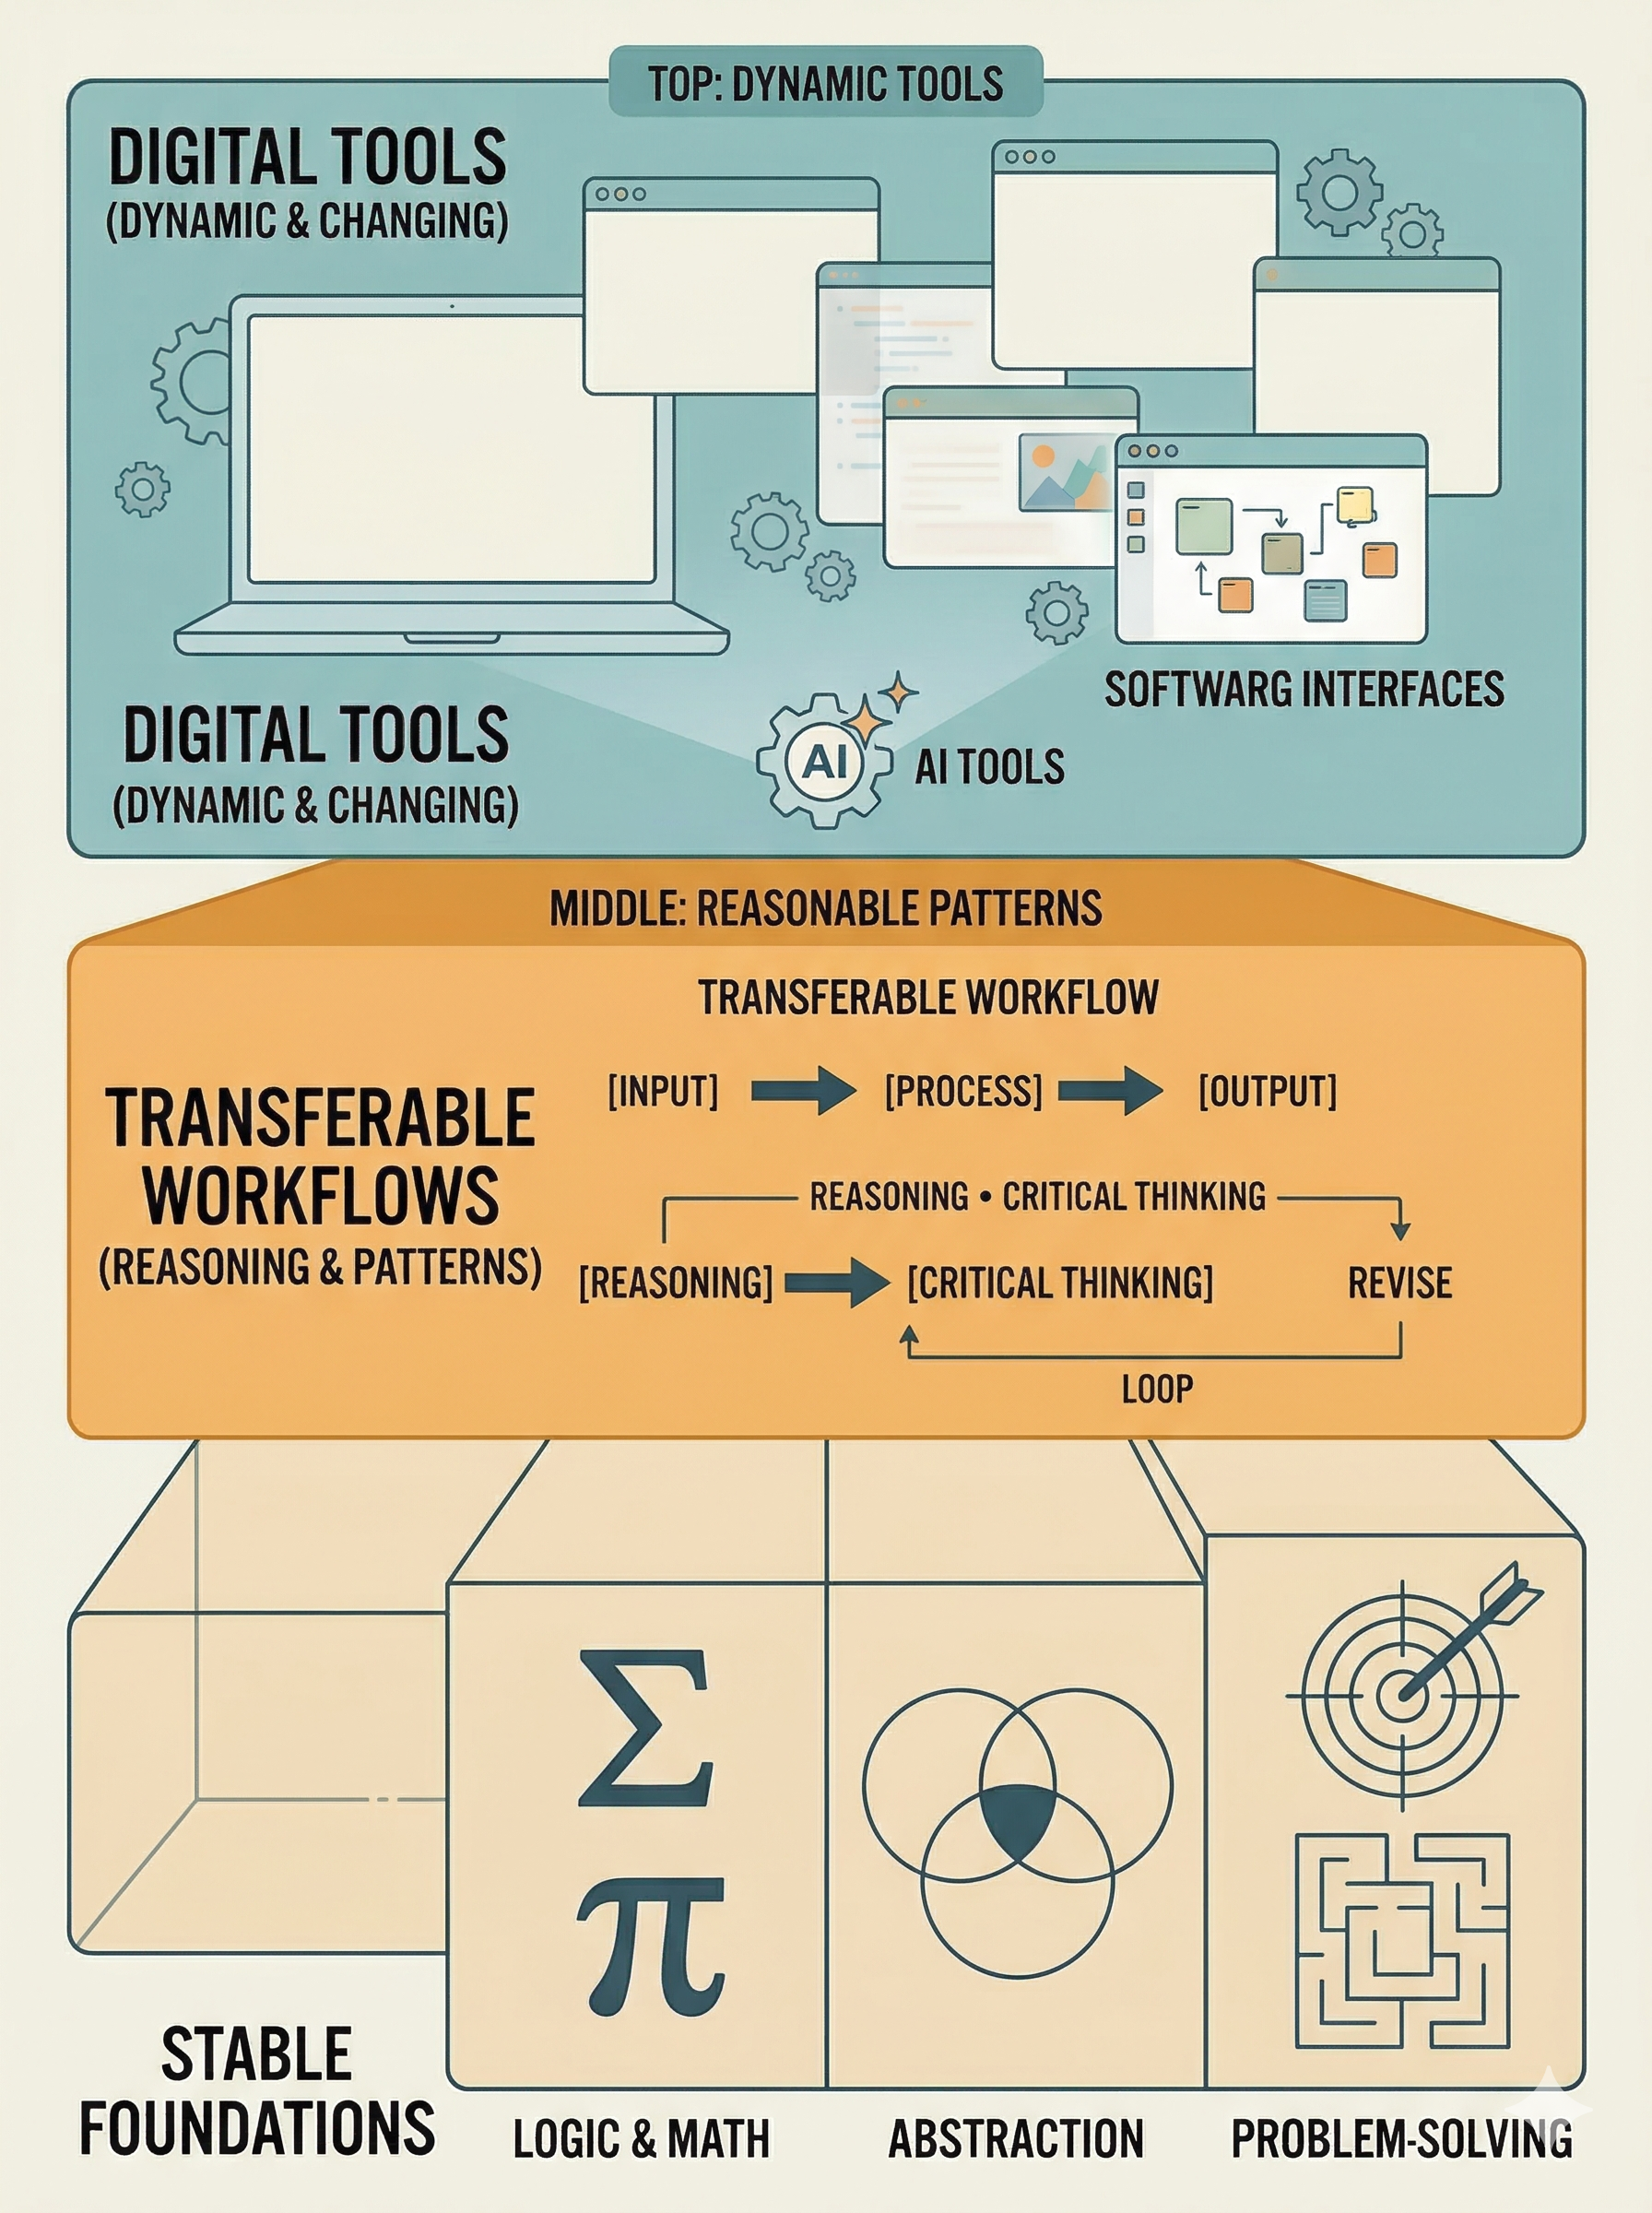
\includegraphics[width=\linewidth,height=0.78\textheight,keepaspectratio]{Gemini_Generated_Image_ToolVSConcept.png}
  \end{columns}
\end{frame}

\section{Counterargument}

\begin{frame}{A Real Tension}
  \begin{columns}[c,totalwidth=\textwidth]
    \column{0.6\textwidth}
    \small
    \begin{itemize}
      \item In the short term, workplaces often reward speed, output, and tool fluency.
      \item So shallow AI use can look efficient at first.
      \item But under heavier AI dependence, checking, exceptions, and accountability matter more.
    \end{itemize}

    \vspace{0.6em}
    \begin{block}{Main Tension}
      \small
      AI speeds up production, but not judgment about what is wrong or risky.
    \end{block}

    \column{0.40\textwidth}
    \centering
    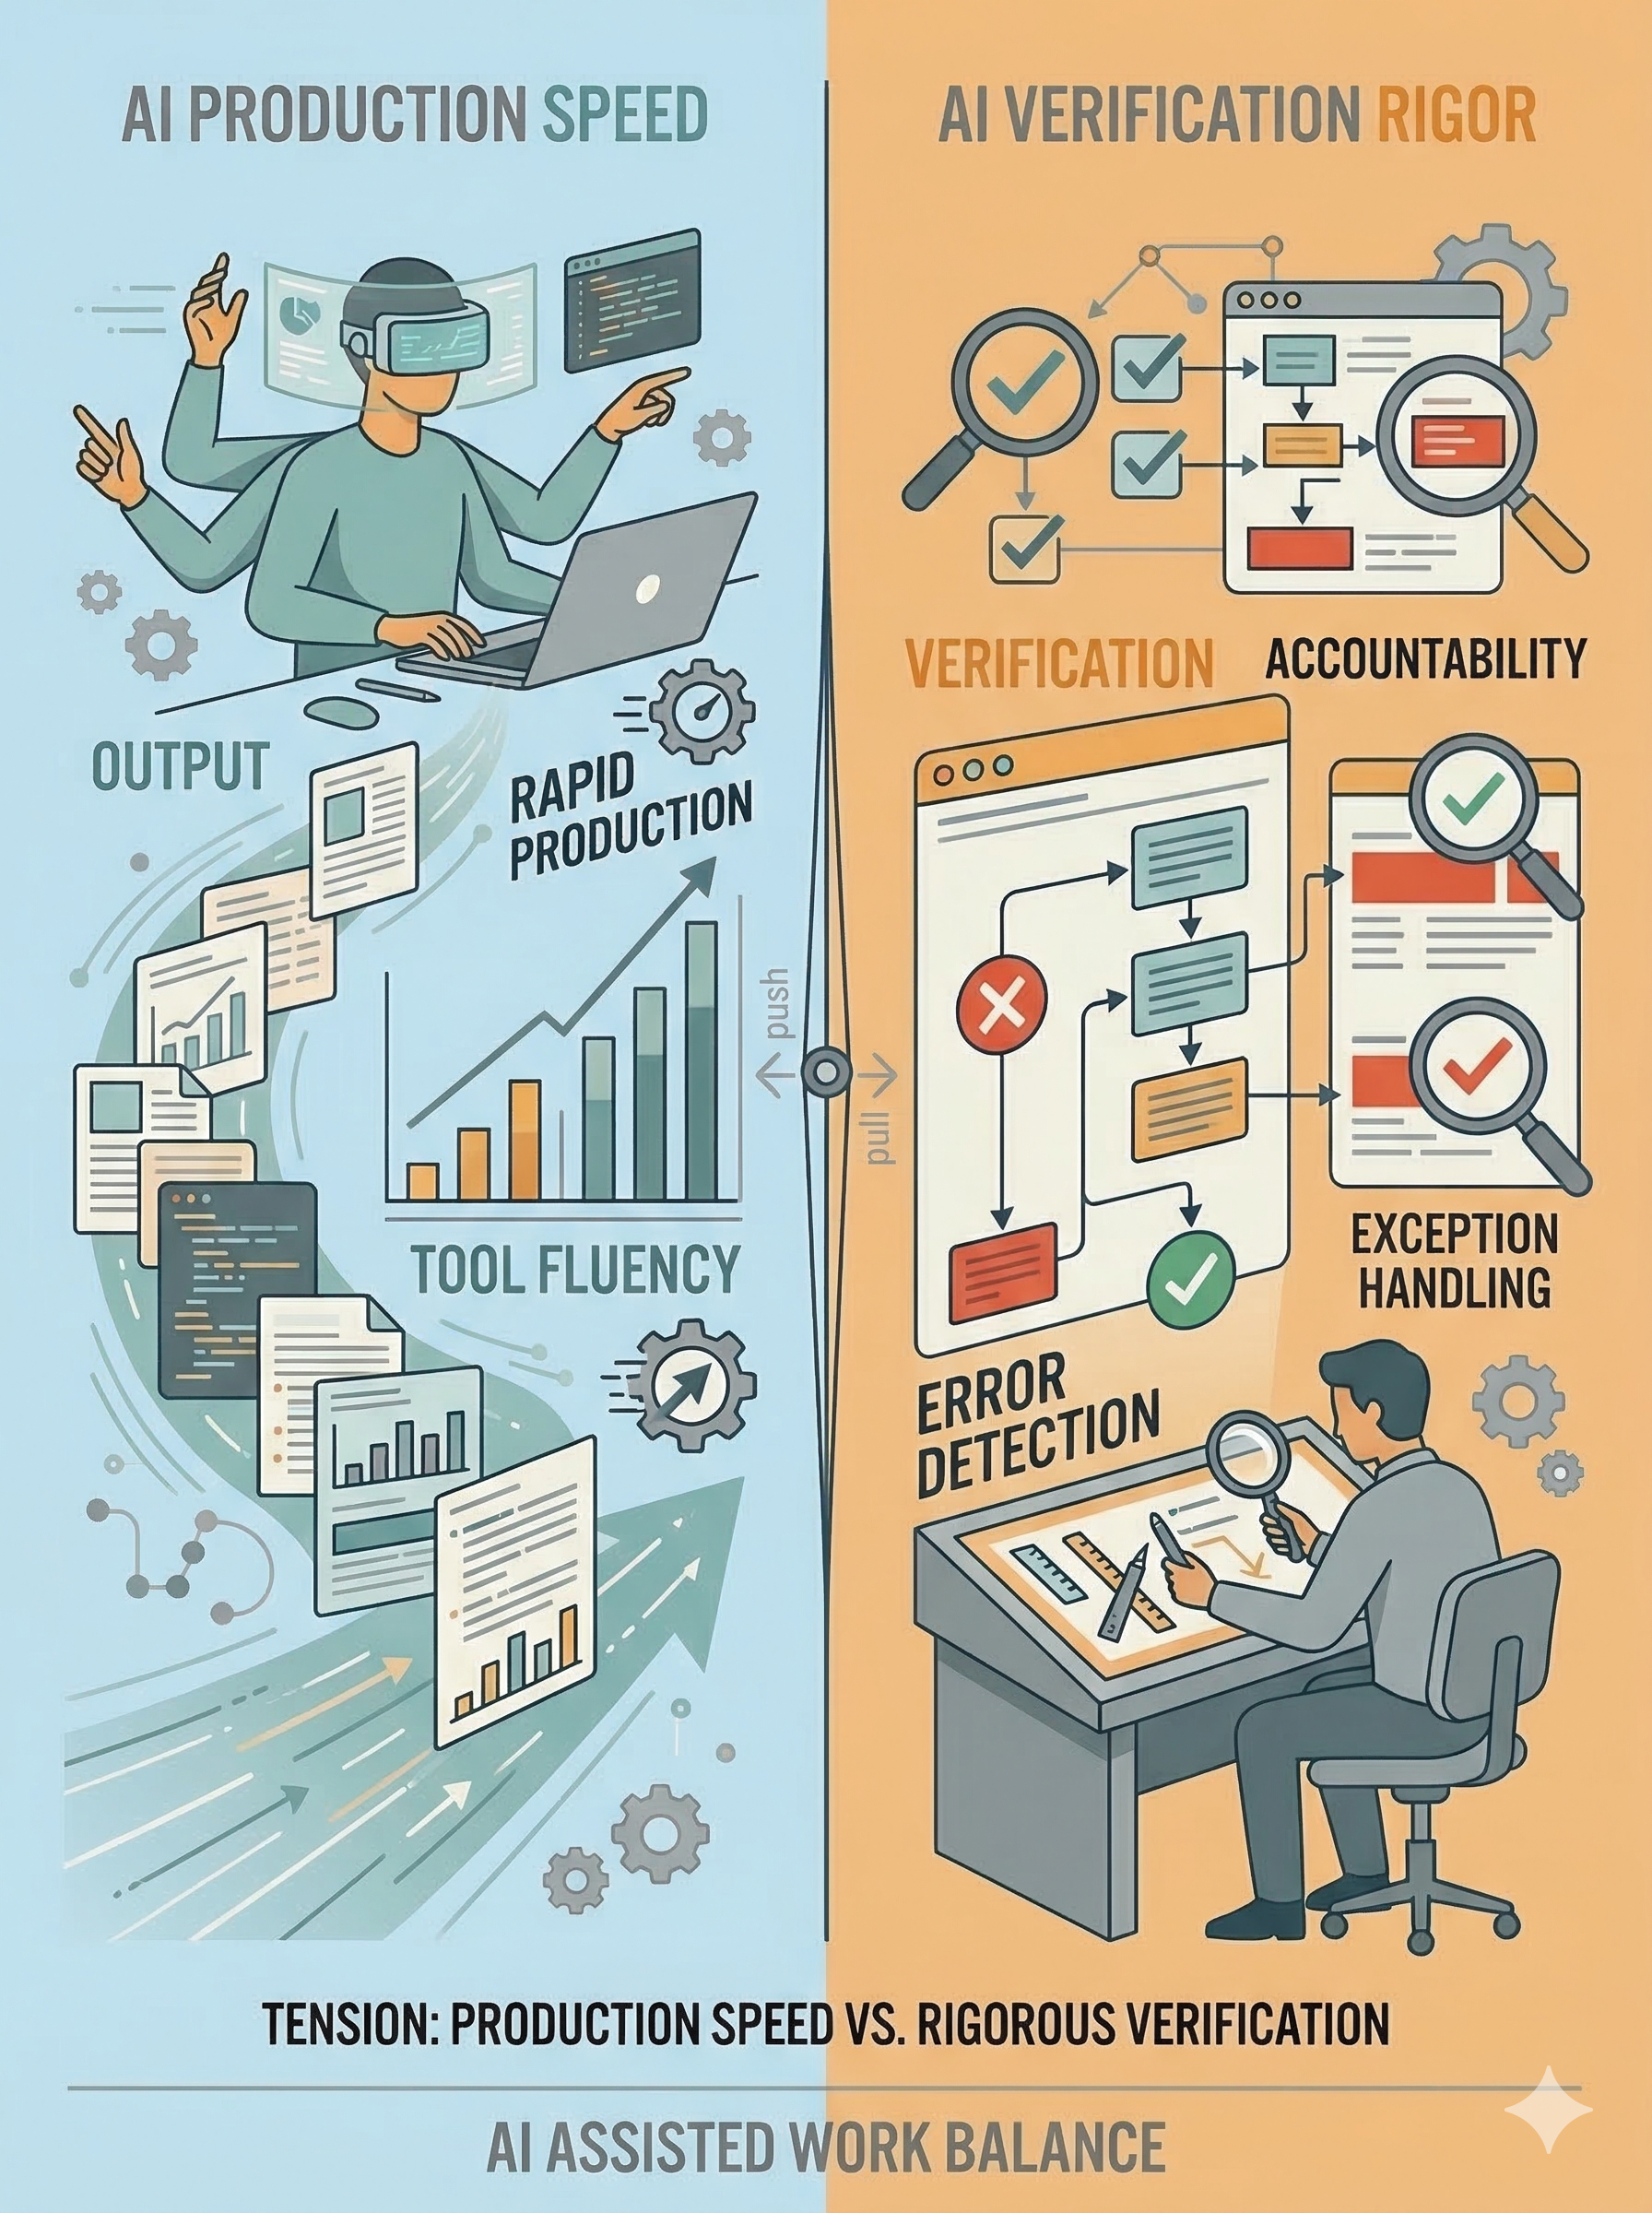
\includegraphics[width=\linewidth,height=0.78\textheight,keepaspectratio]{Gemini_Generated_Image_GenerateVSCheck.png}
  \end{columns}
\end{frame}

\section{Conclusion}

\begin{frame}{Conclusion}
  \begin{itemize}
    \item AI is changing work, but not every change is replacement.
    \item It lowers the cost of retrieval and first-draft generation.
    \item \alert{It does not lower the need for interpretation, verification, and transfer to the same degree.}
    \item The issue is not whether learning disappears, but which forms of understanding become relatively more valuable.
  \end{itemize}
\end{frame}

\section{References}

\begin{frame}[allowframebreaks]{References}
  \footnotesize
  \begin{thebibliography}{9}
    \bibitem{anthropic2026}
    Anthropic.
    \newblock \emph{The Anthropic Economic Index: AI's Impact on Software Development}.
    \newblock March 5, 2026.

    \bibitem{images2026}
    Jianye Shi.
    \newblock Slides illustrations generated with Gemini and adapted for this presentation.
    \newblock 2026.
  \end{thebibliography}
\end{frame}

\begin{frame}{Thank You}
  \centering
  {\LARGE Thank you!}

  \vspace{1em}
  Questions?
\end{frame}

\end{document}
